\section{PROCEDIMIENTO} 

\begin{itemize}
\subsection{Ejercicio 1: Conectando a Power BI a datos}
	\subsubsection{Parte 1: Conectar a datos existentes }

		\item Para realizar los gráficos en PowerBi Desktop primero debemos conectarnos con nuestra base de datos, que ya tiene que tener la base de datos "AdventureWorksLT2016".  Tambien tenemos que tener los archivos de "LabExcercise1.sql" donde se encuentra las Task para cargar los datos en PowerBi. \\Abrimos nuestro PowerBi desktop y procedemos a realizar la conexión a SQL server.
		\begin{figure}[h]
		\begin{center}
		\fbox{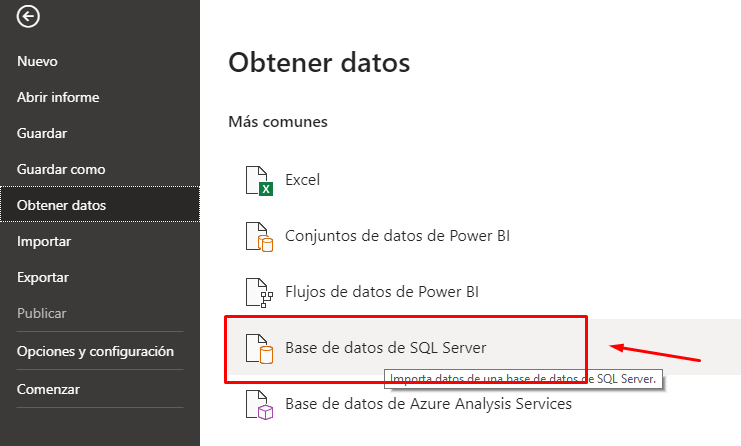
\includegraphics[width=9cm]{./Imagenes/tarea1}}
		\end{center}
		\end{figure}
		\begin{figure}[h]
		\begin{center}
		\fbox{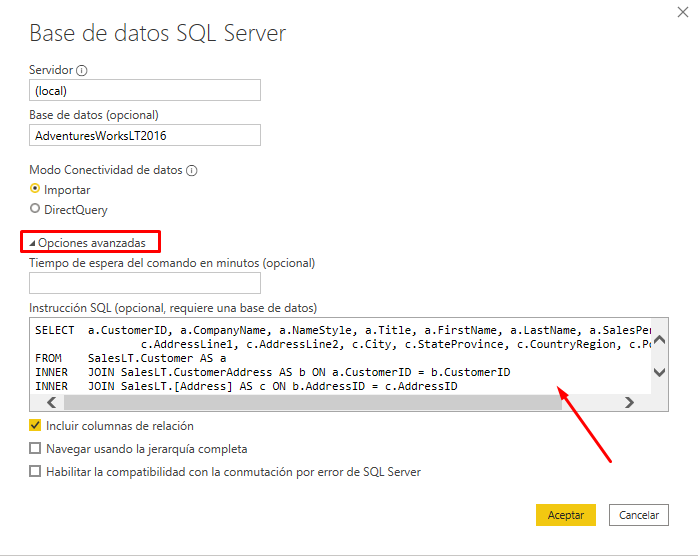
\includegraphics[width=12cm]{./Imagenes/tarea1_1}}
		\end{center}
		\end{figure}
		
\clearpage
		\begin{figure}[h]
		\begin{center}
		\fbox{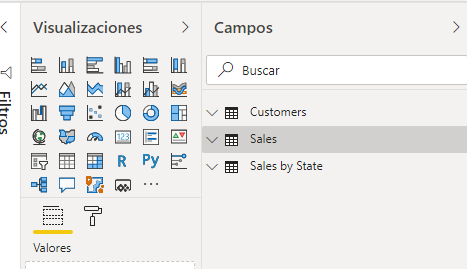
\includegraphics[width=11cm]{./Imagenes/tarea1_3}}
		\end{center}
		\end{figure}

		\item Una vez terminado de cargas los datos que necesitaremos, podremos visualizarlo en el panel lateral derecho de nombre "Campos".	
     \subsubsection{Parte 2: Graficar Datos }
	\item Los datos de cada tabla en la pestaña de "Campos" se va a configurar algunos datos. como el asignarle una categoria a un campo y la creacion de nuevas columnas de datos con los campos que ya tenemos.
\begin{figure}[h]
		\begin{center}
		\fbox{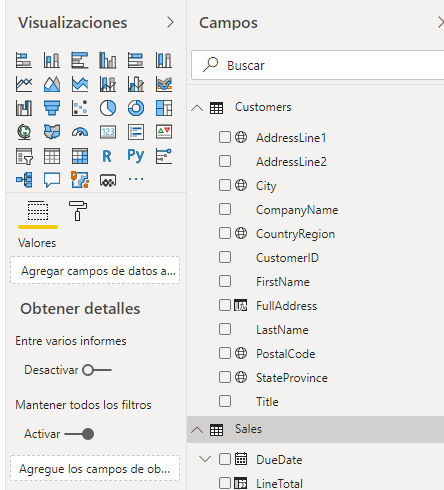
\includegraphics[width=9cm]{./Imagenes/tarea1_2}}
		\end{center}
		\end{figure}
\clearpage
   \subsubsection{Parte 3: Combinar Datos }
	\item En esta parte se combinaran una tabla de "Códigos y abreviaturas de los estados, territorios y otras regiones de los Estados Unidos" que esta en una pagina web, con la tabla de "Sales by State".

\begin{figure}[h]
		\begin{center}
		\fbox{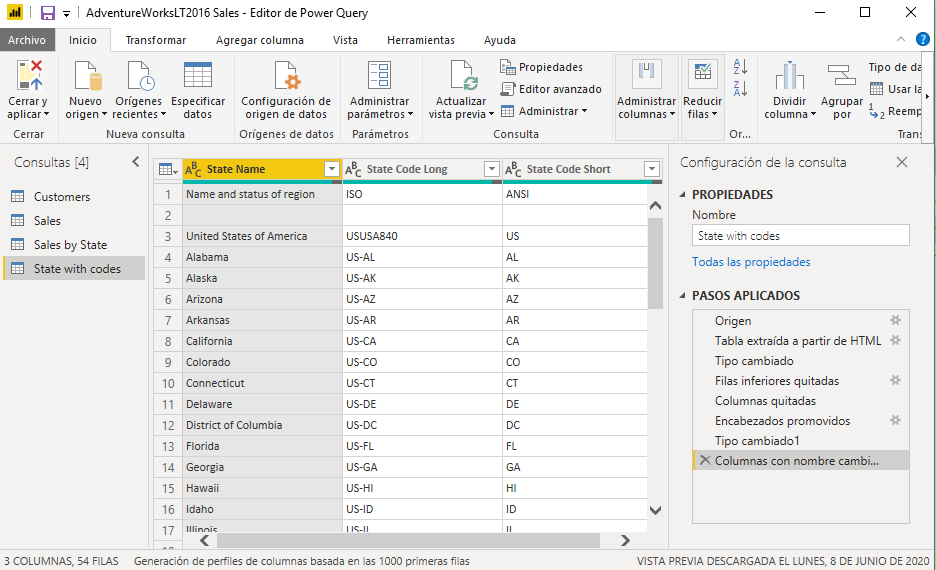
\includegraphics[width=12cm]{./Imagenes/tarea2_1}}
		\end{center}
		\end{figure}

\subsection{Ejercicio 2: : Construyendo Reportes en PowerBI}
\subsubsection{Parte 1: Crear Gráficos }
	\item Realizaremos los gráficos con la información de la base de datos que seleccionamos. Utilizaremos del panel de Visualizaciones los diferentes gráficos que nos ofrecen.

\begin{itemize}
	\item{\textbf{1. Meta de Ventas: }} En el Gráfico de Velocímetro (Gauge) que nos muestra el reporte de la meta de ventas.
	\item {\textbf{2. Ordenes por Categoría Principal: }}En el gráfico de barras apiladas, muestra los la cantidad ordenes por las categorías como: Bicicletas, Ropa, Componentes y Accesorios.
	\item {\textbf{3. Top 10 bicicletas más vendidas: }}En el segundo gráfico de barras apiladas, muestra el top 10 de las bicicletas mas vendidas según su tipo de categoría.
	\item {\textbf{4. Top Selling Customers: }}En el gráfico de Pie o Circular, podremos visualizar el porcentaje y la cifra en dolares de las ventas a los clientes.
	\item {\textbf{5. Ventas por categorías: }}En el gráfico de Donut, podremos visualizar la cantidad de ventas en su total en dólares segun su tipo de categoría como: Bicicletas, Ropa, Componentes y Accesorios. 
	\end{itemize}

\begin{figure}[h]
	\begin{center}
	\fbox{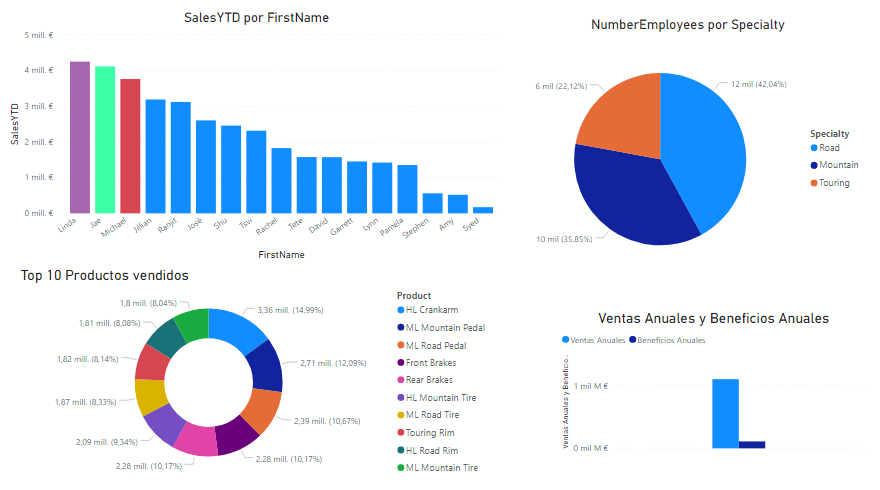
\includegraphics[width=15cm]{./Imagenes/tarea2}}
	\end{center}
	\end{figure}
		

\subsubsection{Parte 2: Crear una Visualización de Mapa}
	\item En esta parte, se crea un mapa con los datos de los Clientes, Ciudades, y las Ventas.
\begin{itemize}
	\item{\textbf{1. Ventas Mundiales por Ciudades: }} En el Gráfico de Mapa, se muestra circulos en las ciudades donde se han realizado ventas a nivel Mundial.
	\item {\textbf{2. Ventas por Estado: }}En el gráfico de Mapa, muestra en forma de circulo en los estados donde se han realizado las ventas.
	\end{itemize}


\begin{figure}[h]
	\begin{center}
	\fbox{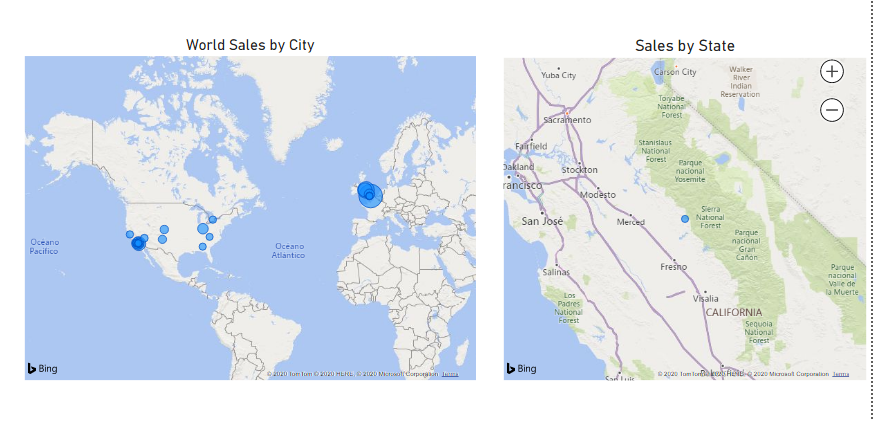
\includegraphics[width=15cm]{./Imagenes/tarea3}}
	\end{center}
	\end{figure}


\end{itemize}
		